% This file contains all the necessary TeX statements for specifying
% overall document format.  This is the file you would edit to set
% any global typesetting parameters.

\input epsf.tex

% This line effectively turns off "Underfull \vbox" error messages.
\vbadness=10000

\tolerance = 1000
\pretolerance = 10000

%%%%%%%%%%%%%%%%%%%%%%%%%%%%%%%%%%%%%%%%%%%%%%%%%%%%%%%%%%%%%%%%%%%%%%%%%%%%%
\vskip 5pt \hrule \vskip 5pt \noindent {\bf Question 21} -- LIII (fluid viscosity) \vskip 10pt

Viscosity is a measure of a fluid's resistance to {\it shear}.  It may be thought of as a fluid's ``internal friction''.

\vskip 10pt

Absolute viscosity is defined in terms of shear force versus shear velocity, and is symbolized by the Greek letters ``eta'' ($\eta$) or ``mu'' ($\mu$).  The unit of measurement for absolute viscosity is the Pascal-second, or the {\it poise} (0.1 Pascal-seconds).  Water has an absolute viscosity of 1 centipoise (1 cp).

\vskip 10pt

Kinematic viscosity is defined in terms of absolute viscosity per unit density, and is symbolized by the Greek letter ``nu'' ($\nu$).  The unit of measurement for kinematic viscosity is the {\it stokes}, defined as one poise of absolute viscosity for a mass density of 1 gram per cubic centimeter.  Water has a kinematic viscosity of 1 centistokes.

\vskip 10pt

The mechanism of liquid viscosity is inter-molecular {\it cohesion}.  Thus, increasing temperature typically reduces the viscosity of liquids.  The mechanism of gas viscosity is inter-molecular {\it collision}.  Thus increasing temperature typically increases the viscosity of gases.

\vskip 10pt

Some fluids -- called non-Newtonian fluids -- exhibit viscosity changes with changes in applied stress.  A mixture of cornstarch and water is one example of a non-Newtonian fluid because it tends to ``solidify'' when stress is applied.


%%%%%%%%%%%%%%%%%%%%%%%%%%%%%%%%%%%%%%%%%%%%%%%%%%%%%%%%%%%%%%%%%%%%%%%%%%%%%
\filbreak \vskip 5pt \hrule \vskip 5pt \noindent {\bf Question 22} -- LIII (Reynolds number) \vskip 10pt

Reynolds number is a unitless measure of a fluid's momentum versus its viscosity (a ratio of kinetic forces to viscous forces).  Low Reynolds numbers predict ``viscid'' or {\it laminar} flow, where the paths of fluid molecules travel in straight lines with little or no intersection.  High Reynolds numbers predict ``inviscid'' or {\it turbulent} flow, where fluid molecules move chaotically with lots of intersection and mixing on a microscopic scale.  This kind of micro-turbulent flow is not to be confused with large-scale turbulence such as swirls and eddies caused by piping irregularities.

\vskip 10pt

Turbulent flow is often desired in industrial processes such as heat exchange, mixing, and flow measurement.  Microscopic turbulence has the effect of ``flattening'' the flow profile of fluid exhibiting swirls and other large-scale turbulence from piping shapes -- in other words, micro-turbulence helps condition the flow for good flow measurement.

\vskip 10pt

Reynolds values less than 2000 are usually associated with laminar flow.  Values in excess of 10000 are usually associated with turbulent flow.


%%%%%%%%%%%%%%%%%%%%%%%%%%%%%%%%%%%%%%%%%%%%%%%%%%%%%%%%%%%%%%%%%%%%%%%%%%%%%
\filbreak \vskip 5pt \hrule \vskip 5pt \noindent {\bf Question 23} -- LIII (Law of Continuity) \vskip 10pt

The Law of Mass Conservation dictates that the mass flow rate through a pipe having no leaks or pulsations in the flow stream must remain constant, like current in a series circuit.  This mass flow rate is equal to the mass density of the fluid ($\rho$) multiplied by the cross-sectional area of the pipe ($A$) multiplied by the average velocity of the fluid ($\overline{v}$):

$$W = \rho A \overline{v}$$

In situations where the fluid is ``incompressible'' (i.e. does not exhibit substantial changes in density), the $\rho$ term may be ignored, and constant volumetric flow ($Q$) assumed at all places in a pipe:

$$Q = A \overline{v}$$

This tells us that the velocity of a fluid will be inversely proportional to the cross-sectional area of the pipe: if the pipe gets skinnier, the velocity increases.


%%%%%%%%%%%%%%%%%%%%%%%%%%%%%%%%%%%%%%%%%%%%%%%%%%%%%%%%%%%%%%%%%%%%%%%%%%%%%
\filbreak \vskip 5pt \hrule \vskip 5pt \noindent {\bf Question 24} -- flow velocity calculations \vskip 10pt

$$Q = A \overline{v}$$

Average flow velocity through the 8 inch pipe:

$$\overline{v} = {Q \over A} = {70 \hbox{ ft}^3/\hbox{min} \over 0.3474 \hbox{ ft}^2} = 201.49 \hbox{ ft/min}$$

\vskip 10pt

Average flow velocity through the 2.5 inch pipe:

$$\overline{v} = {Q \over A} = {70 \hbox{ ft}^3/\hbox{min} \over 0.03325 \hbox{ ft}^2} = 2105.4 \hbox{ ft/min}$$

\vskip 10pt

$$\left({70 \hbox{ ft}^3 \over \hbox{min}}\right) \left({1728 \hbox{ in}^3 \over \hbox{ft}^3}\right) \left({1 \hbox{ gal} \over 231 \hbox{ in}^3} \right) = 523.64 \hbox{ GPM}$$


%%%%%%%%%%%%%%%%%%%%%%%%%%%%%%%%%%%%%%%%%%%%%%%%%%%%%%%%%%%%%%%%%%%%%%%%%%%%%
\filbreak \vskip 5pt \hrule \vskip 5pt \noindent {\bf Question 25} -- Reynolds number calculation \vskip 10pt

$$\hbox{Re} = {{3160 G_f Q} \over {D \mu}}$$

\noindent
Where,

Re = Reynolds number (unitless)

$G_f$ = Specific gravity of liquid (unitless)

$Q$ = Flow rate (gallons per minute)

$D$ = Diameter of pipe (inches)

$\mu$ = Absolute viscosity of fluid (centipoise)

3160 = Conversion factor for British units

\vskip 10pt


$$Q = {\hbox{Re} D \mu \over 3160 G_f}$$

$$Q = {(12500) (6.065) (111) \over (3160) \left(57.3 \over 62.4\right)} = 2900.1 \hbox{ GPM}$$

$Q$ (minimum) = 2900.1 GPM = 387.7 ft$^{3}$/min {\it (which is an extraordinarily high flow rate for a 6-inch pipe!)}

\vskip 10pt

$$Q = A \overline{v}$$

$$\overline{v} = {Q \over A} = {387.7 \hbox{ ft}^3\hbox{/min} \over 0.2006 \hbox{ ft}^2} = 1932.35 \hbox{ ft/min}$$

\vskip 10pt

Based on these large figures, this might not be the best flowmeter technology to use on olive oil!  The relatively high viscosity of the oil makes it difficult to achieve the requisite Reynolds number for good operation.


%%%%%%%%%%%%%%%%%%%%%%%%%%%%%%%%%%%%%%%%%%%%%%%%%%%%%%%%%%%%%%%%%%%%%%%%%%%%%
\filbreak \vskip 5pt \hrule \vskip 5pt \noindent {\bf Question 26} -- LIII (Bernoulli's equation) \vskip 10pt

If the flow of fluid through a pipe is inviscid (free of viscous forces dissipating energy via friction) and there is no pump or valve or other energy-translating device placed in the stream, we may safely assume the energy of that fluid remains constant at it travels through different portions of the piping system.  This is a consequence of the Law of Energy Conservation, and is expressed in Bernoulli's equation which specifies the total energy in a fluid stream in three ``heads'' (elevation, velocity, and pressure):

$$z_1 \rho g + {v_1^2 \rho \over 2} + P_1 = z_2 \rho g + {v_2^2 \rho \over 2} + P_2$$

$$z_1 + {v_1^2 \over {2 g}} + {P_1 \over \gamma} = z_2 + {v_2^2 \over {2 g}} + {P_2 \over \gamma}$$

\noindent
Where,

$z$ = Height of fluid (from a common reference point, usually ground level)

$\rho$ = Mass density of fluid

$\gamma$ = Weight density of fluid ($\gamma = \rho g$)

$g$ = Acceleration of gravity

$v$ = Velocity of fluid

$P$ = Pressure of fluid

\vskip 10pt

Potential energy in the form of liquid elevation above ground level ($z \rho g$) is analogous to potential energy of a raised mass ($mgh$).  Kinetic energy in the form of liquid velocity ($\rho v^2 \over 2$) is analagous to kinetic energy of a moving mass (${1 \over 2} mv^2$).  Potential energy of a fluid expressed as a {\it pressure} ($P$) has no direct analogue in the world of solids.

\vskip 10pt

It is critically important that all units are kept consistent when applying Bernoulli's equation to real flow applications.  If velocity is expressed in feet per second, then pressure must be expressed in pounds per square feet, gravity in feet per second squared, and density in slugs per cubic foot.

\vskip 10pt

The relationship between weight density ($\gamma$) and mass density ($\rho$) is given by the following formula:

$$\gamma = \rho g$$

$g$ is the acceleration of Earth's gravity expressed as 32.2 feet per second squared, or 9.81 meters per second squared.


%%%%%%%%%%%%%%%%%%%%%%%%%%%%%%%%%%%%%%%%%%%%%%%%%%%%%%%%%%%%%%%%%%%%%%%%%%%%%
\filbreak \vskip 5pt \hrule \vskip 5pt \noindent {\bf Question 27} -- LIII (flow through a venturi tube) \vskip 10pt

As fluid moves through a venturi tube (a tube that narrows and then expands back to its former diameter), the fluid must accelerate through the constriction.  This increases the kinetic energy of the fluid molecules as they pass through the constriction.  As kinetic energy increases, potential energy of the fluid molecules must decrease at the same time, resulting in a decrease in pressure at the venturi tube's throat.

\vskip 10pt

The fluid pressure mostly ``recovers'' as it slows back down in the tail of the venturi tube.  Some pressure is lost permenantly, due to frictional energy losses through the venturi tube, but this is usually minimal.

\vskip 10pt

If peizometer tubes and pitot tubes are installed in am ideal venturi, the pressure and velocity heads may be shown by the liquid heights inside those tubes:

$$\epsfxsize=3in \includegraphics[width=15.5cm]{i04036x01.eps}$$

$$z_1 + {v_1^2 \over {2 g}} + {P_1 \over \gamma} = z_2 + {v_2^2 \over {2 g}} + {P_2 \over \gamma} = z_3 + {v_3^2 \over {2 g}} + {P_3 \over \gamma}$$


%%%%%%%%%%%%%%%%%%%%%%%%%%%%%%%%%%%%%%%%%%%%%%%%%%%%%%%%%%%%%%%%%%%%%%%%%%%%%
\filbreak \vskip 5pt \hrule \vskip 5pt \noindent {\bf Question 28} -- steam eductor in realistic P\&ID \vskip 10pt

Vacuum is produced through the use of a {\it steam eductor}, where the throat of a venturi tube passing steam connects to the tank, sucking in vapors from the tank and into the steam flow.  

\vskip 10pt

In order to halt the production of vacuum, operators must halt the flow of steam through the eductor.

\vskip 10pt

The level instrument (LT-18) is a pressure-sensing instrument measuring the hydrostatic pressure at the bottom of the tank.  LG-19 is a tape-and-float instrument.


%%%%%%%%%%%%%%%%%%%%%%%%%%%%%%%%%%%%%%%%%%%%%%%%%%%%%%%%%%%%%%%%%%%%%%%%%%%%%
\filbreak \vskip 5pt \hrule \vskip 5pt \noindent {\bf Question 29} -- Bernoulli's equation calculation \vskip 10pt

% No blank lines allowed between lines of an \halign structure!
% I use comments (%) instead, so Tex doesn't choke.

$$\vbox{\offinterlineskip
\halign{\strut
\vrule \quad\hfil # \ \hfil & 
\vrule \quad\hfil # \ \hfil & 
\vrule \quad\hfil # \ \hfil \vrule \cr
\noalign{\hrule}
%
% First row
{\bf Head} & {\bf Calculation} at 12 inch pipe & {\bf Value} \cr
%
\noalign{\hrule}
%
% Another row
$z_1 \rho g$ & (0 ft) (1.951 slugs/ft$^{3}$) (32.2 ft/s$^{2}$) & 0 lb/ft$^{2}$ \cr
%
\noalign{\hrule}
%
% Another row
$v_1^2 \rho / 2$ & (9.549 ft/s)$^{2}$ (1.951 slugs/ft$^{3}$) / 2 & 88.955 lb/ft$^{2}$ \cr
%
\noalign{\hrule}
%
% Another row
$P_1$ & (80 lb/in$^{2}$) (144 in$^{2}$/1 ft$^{2}$) & 11520 lb/ft$^{2}$ \cr
%
\noalign{\hrule}
%
% Another row
{\bf Total} &  0 lb/ft$^{2}$ + 88.955 lb/ft$^{2}$ + 11520 lb/ft$^{2}$ & {\bf 11608.955 lb/ft$^{2}$} \cr
%
\noalign{\hrule}
} % End of \halign 
}$$ % End of \vbox

\vskip 10pt

% No blank lines allowed between lines of an \halign structure!
% I use comments (%) instead, so Tex doesn't choke.

$$\vbox{\offinterlineskip
\halign{\strut
\vrule \quad\hfil # \ \hfil & 
\vrule \quad\hfil # \ \hfil & 
\vrule \quad\hfil # \ \hfil \vrule \cr
\noalign{\hrule}
%
% First row
{\bf Head} & {\bf Calculation} at 5 inch pipe & {\bf Value} \cr
%
\noalign{\hrule}
%
% Another row
$z_2 \rho g$ & (0 ft) (1.951 slugs/ft$^{3}$) (32.2 ft/s$^{2}$) & 0 lb/ft$^{2}$ \cr
%
\noalign{\hrule}
%
% Another row
$v_2^2 \rho / 2$ & (55.004 ft/s)$^{2}$ (1.951 slugs/ft$^{3}$) / 2 & 2951.31 lb/ft$^{2}$ \cr
%
\noalign{\hrule}
%
% Another row
$P_2$ & (?? lb/in$^{2}$) (144 in$^{2}$/1 ft$^{2}$) & ??? lb/ft$^{2}$ \cr
%
\noalign{\hrule}
%
% Another row
{\bf Total} &  0 lb/ft$^{2}$ + 2951.31 lb/ft$^{2}$ + ??? lb/ft$^{2}$ & {\bf 11608.955 lb/ft$^{2}$} \cr
%
\noalign{\hrule}
} % End of \halign 
}$$ % End of \vbox

$$P_2 = 11608.955 \hbox{ lb/ft}^2 - 2951.31 \hbox{ lb/ft}^2 = 8657.64 \hbox{ lb/ft}^2 = 60.123 \hbox{ PSI}$$

\vskip 10pt

$\Delta P$ = $P_1 - P_2$ = 80 PSI $-$ 60.123 PSI = 19.877 PSI


%%%%%%%%%%%%%%%%%%%%%%%%%%%%%%%%%%%%%%%%%%%%%%%%%%%%%%%%%%%%%%%%%%%%%%%%%%%%%
\filbreak \vskip 5pt \hrule \vskip 5pt \noindent {\bf Question 30} -- Bernoulli's equation calculation \vskip 10pt

% No blank lines allowed between lines of an \halign structure!
% I use comments (%) instead, so Tex doesn't choke.

$$\vbox{\offinterlineskip
\halign{\strut
\vrule \quad\hfil # \ \hfil & 
\vrule \quad\hfil # \ \hfil & 
\vrule \quad\hfil # \ \hfil \vrule \cr
\noalign{\hrule}
%
% First row
{\bf Head} & {\bf Calculation} at 12 inch pipe & {\bf Value} \cr
%
\noalign{\hrule}
%
% Another row
$z_1 \rho g$ & (0 ft) (1.951 slugs/ft$^{3}$) (32.2 ft/s$^{2}$) & 0 lb/ft$^{2}$ \cr
%
\noalign{\hrule}
%
% Another row
$v_1^2 \rho / 2$ & (19.098 ft/s)$^{2}$ (1.951 slugs/ft$^{3}$) / 2 & 355.820 lb/ft$^{2}$ \cr
%
\noalign{\hrule}
%
% Another row
$P_1$ & (80 lb/in$^{2}$) (144 in$^{2}$/1 ft$^{2}$) & 11520 lb/ft$^{2}$ \cr
%
\noalign{\hrule}
%
% Another row
{\bf Total} &  0 lb/ft$^{2}$ + 355.820 lb/ft$^{2}$ + 11520 lb/ft$^{2}$ & {\bf 11875.820 lb/ft$^{2}$} \cr
%
\noalign{\hrule}
} % End of \halign 
}$$ % End of \vbox

\vskip 10pt

% No blank lines allowed between lines of an \halign structure!
% I use comments (%) instead, so Tex doesn't choke.

$$\vbox{\offinterlineskip
\halign{\strut
\vrule \quad\hfil # \ \hfil & 
\vrule \quad\hfil # \ \hfil & 
\vrule \quad\hfil # \ \hfil \vrule \cr
\noalign{\hrule}
%
% First row
{\bf Head} & {\bf Calculation} at 5 inch pipe & {\bf Value} \cr
%
\noalign{\hrule}
%
% Another row
$z_2 \rho g$ & (0 ft) (1.951 slugs/ft$^{3}$) (32.2 ft/s$^{2}$) & 0 lb/ft$^{2}$ \cr
%
\noalign{\hrule}
%
% Another row
$v_2^2 \rho / 2$ & (110.01 ft/s)$^{2}$ (1.951 slugs/ft$^{3}$) / 2 & 11805.245 lb/ft$^{2}$ \cr
%
\noalign{\hrule}
%
% Another row
$P_2$ & (?? lb/in$^{2}$) (144 in$^{2}$/1 ft$^{2}$) & ??? lb/ft$^{2}$ \cr
%
\noalign{\hrule}
%
% Another row
{\bf Total} &  0 lb/ft$^{2}$ + 11805.245 lb/ft$^{2}$ + ??? lb/ft$^{2}$ & {\bf 11875.820 lb/ft$^{2}$} \cr
%
\noalign{\hrule}
} % End of \halign 
}$$ % End of \vbox

$$P_2 = 11875.820 \hbox{ lb/ft}^2 - 11805.245 \hbox{ lb/ft}^2 = 70.575 \hbox{ lb/ft}^2 = 0.4901 \hbox{ PSI}$$

\vskip 10pt

If the second version of Bernoulli's equation is used, you get a slightly different result for $P_2$ of 0.531 PSI instead of 0.490 PSI.  The difference between the two answers lies in the imperfect equivalence of 1.951 slugs/ft$^{3}$ (mass density) and 62.4 lb/ft$^{3}$ (weight density) for water.

\vskip 10pt

$\Delta P$ = $P_1 - P_2$ = 80 PSI $-$ 0.4901 PSI = 79.510 PSI


%%%%%%%%%%%%%%%%%%%%%%%%%%%%%%%%%%%%%%%%%%%%%%%%%%%%%%%%%%%%%%%%%%%%%%%%%%%%%
\filbreak \vskip 5pt \hrule \vskip 5pt \noindent {\bf Summary questions and review of general principles} \vskip 10pt

\noindent
Identify any general principles you've learned today (i.e. principles spanning multiple applications).
\item{$\bullet$} Law of Mass Conservation: mass cannot be created or destroyed, but must be accounted
\item{$\bullet$} Law of Energy Conservation: energy cannot be created or destroyed, but must be accounted
\item{$\bullet$} Flow through a venturi tube creates a decrease in pressure, possibly all the way to a vacuum state (less than atmospheric pressure!)
\medskip

\begin{itemize}
\item{$(Q21)$} Summarize main points of the reading (viscosity)
\item{$(Q22)$} Summarize main points of the reading (Reynolds number)
\item{$(Q23)$} Summarize main points of the reading (Law of Continuity)
\item{$(Q24)$} Show mathematical work calculating velocities and flow in GPM
\item{$(Q25)$} Show mathematical work calculating flow rate and velocity of olive oil
\item{$(Q26)$} Summarize main points of the reading (Bernoulli's equation)
\item{$(Q26)$} Explain {\it why} Bernoilli's equation is true
\item{$(Q26)$} Identify a practical application where we could not apply Bernoulli's equation to two different points in a piping system
\item{$(Q27)$} Summarize main points of the reading (flow through a venturi)
\medskip

\begin{itemize}
\item{$(Q29)$} Show mathematical work using Bermoulli's equation
\item{$(Q30)$} Show mathematical work using Bermoulli's equation
\medskip


%%%%%%%%%%%%%%%%%%%%%%%%%%%%%%%%%%%%%%%%%%%%%%%%%%%%%%%%%%%%%%%%%%%%%%%%%%%%%
\filbreak \vskip 5pt \hrule \vskip 5pt \noindent {\bf Problem Solving question $(Q28)$} \vskip 10pt

Imagine the pressure safety valve PSV-355 stuck open!

\vskip 10pt

PG-316 is registering much less vacuum than is normally expected, despite FI-37 registering a normal amount of steam flow through the eductor.

%$$\epsfxsize=2in \includegraphics[width=15.5cm]{i00000x01.eps}$$


\bye



